\documentclass{beamer}
\setbeamertemplate{navigation symbols}{}
\usepackage{comment}

\setbeamercolor{frametitle}{fg=black,bg=white}
\setbeamercolor{title}{fg=black,bg=yellow!85!orange}
\usetheme{AnnArbor}

\usepackage{textpos} % package for the positioning
\usepackage{listings}
\usepackage{xcolor}
\usepackage[most]{tcolorbox}
\usepackage{mathtools}
\usepackage{graphicx}
\usepackage{graphbox}
\usepackage{movie15}
\usepackage{caption}
\DeclareCaptionType{code}[Code Listing][List of Code Listings] 

\definecolor{codegreen}{rgb}{0,0.6,0}
\definecolor{codegray}{rgb}{0.5,0.5,0.5}
\definecolor{codepurple}{rgb}{0.58,0,0.82}
\definecolor{backcolour}{rgb}{0.95,0.95,0.92} 
\lstdefinestyle{mystyle}{
    backgroundcolor=\color{backcolour},   
    commentstyle=\color{codegreen},
    keywordstyle=\color{magenta},
    numberstyle=\tiny\color{codegray},
    stringstyle=\color{codepurple},
    basicstyle=\ttfamily\footnotesize,
    breakatwhitespace=false,         
    breaklines=true,                 
    captionpos=b,                    
    keepspaces=true,                 
    numbers=left,                    
    numbersep=5pt,                  
    showspaces=false,                
    showstringspaces=false,
    showtabs=false,                  
    tabsize=2
}

\lstset{style=mystyle}

\lstdefinelanguage
   [x64]{Assembler}     % add a "x64" dialect of Assembler
   [x86masm]{Assembler} % based on the "x86masm" dialect
   % with these extra keywords:
   {morekeywords={CDQE,CQO,CMPSQ,CMPXCHG16B,JRCXZ,LODSQ,MOVSXD, %
                  POPFQ,PUSHFQ,SCASQ,STOSQ,IRETQ,RDTSCP,SWAPGS, %
                  rax,rdx,rcx,rbx,rsi,rdi,rsp,rbp, %
                  r8,r8d,r8w,r8b,r9,r9d,r9w,r9b, %
                  r10,r10d,r10w,r10b,r11,r11d,r11w,r11b, %
                  r12,r12d,r12w,r12b,r13,r13d,r13w,r13b, %
                  r14,r14d,r14w,r14b,r15,r15d,r15w,r15b}} %


\beamersetuncovermixins{\opaqueness<1>{25}}{\opaqueness<2->{15}}

%Copyright
\addtobeamertemplate{frametitle}{}{%
\begin{textblock*}{50mm}(0cm,-1.25cm)
\color{yellow!85!orange}
\tiny{Copyright \copyright 2024 CNM.}
\end{textblock*}}

% position the logo
\addtobeamertemplate{frametitle}{}{%
\begin{textblock*}{100mm}(11.4cm,-1.3cm)

\includegraphics[height=1cm,width=1cm,keepaspectratio]{fig/ddclogotransparent.png}
\end{textblock*}}

\AtBeginSection[]{
  \begin{frame}
  \vfill
  \centering
  \begin{beamercolorbox}[sep=8pt,center,shadow=true,rounded=true]{title}
    \usebeamerfont{title}\insertsectionhead\par%
  \end{beamercolorbox}
  \vfill
  \end{frame}
}

\begin{document}
\title{Quantum Workforce Development}
\author{Brian Rashap}
\date{July 2023} 

\begin{frame}
\titlepage
\end{frame}


\section{Geometric Optics}

\begin{frame}\frametitle{Ray Nature of Light}
The word "ray" means a straight line that originates at some point.

\begin{center}
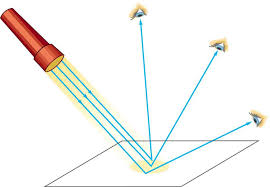
\includegraphics[width=6cm]{fig/rays.jpg}
\end{center}

The part of optics dealing with the ray aspect of light is called "geometric optics."

\end{frame}


\begin{frame}\frametitle{Reflection}
The angle of reflection equals the angle of incidences

\begin{center}
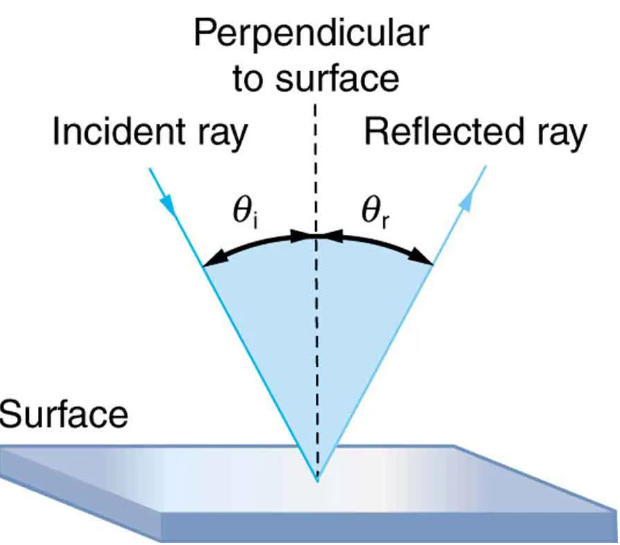
\includegraphics[width=6cm]{fig/reflect.png}
\end{center}

\end{frame}


\begin{frame}\frametitle{Rough vs Smooth Surfaces}

\begin{center}
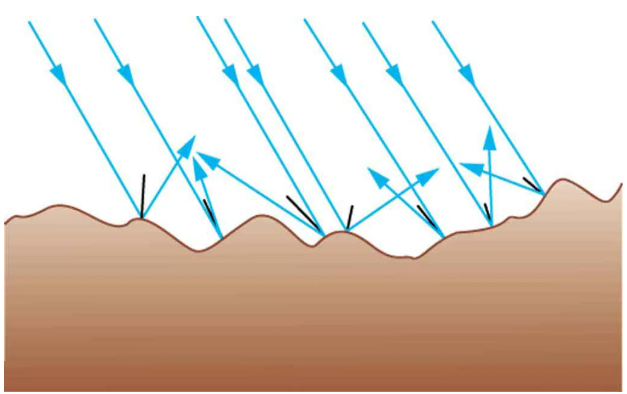
\includegraphics[width=3.5cm]{fig/reflect_rough.png}
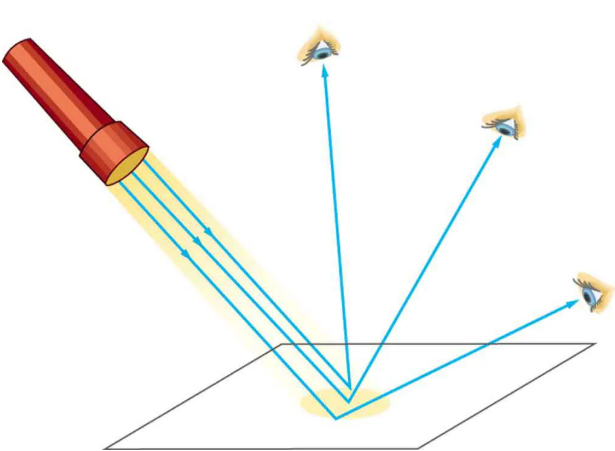
\includegraphics[width=3.5cm]{fig/reflect_paper.png}
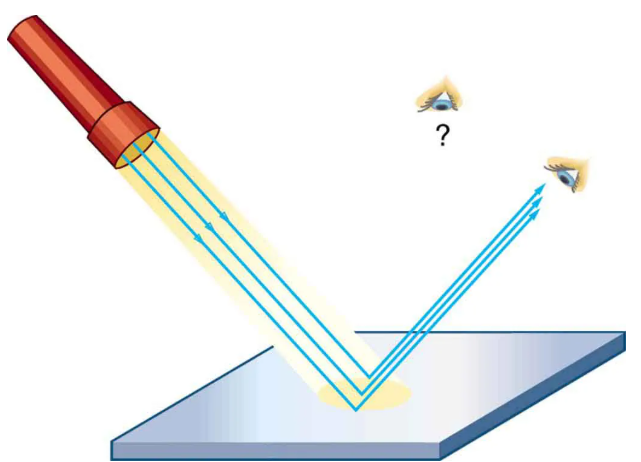
\includegraphics[width=3.5cm]{fig/reflect_mirror.png}
\end{center}

\end{frame}

\begin{frame}\frametitle{Mirrors and Virtual Images}
When we see ourselves in a mirror, it appears that our image is actually behind the mirror.

\begin{center}
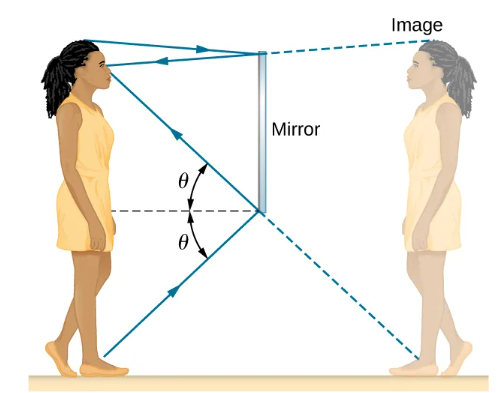
\includegraphics[width=6cm]{fig/virtual.png}
\end{center}

\end{frame}

\begin{frame}\frametitle{Speed of Light}
\begin{columns}
\begin{column}{7cm}
\begin{itemize}
\item In 1676, Danish astronomer Ole Roemer noted the change in orbital period of Jupiter's moons depending of if the earth was moving towards or away from Jupiter. He as able to calculate speed of light to be $2.26 x 10^8 (\frac{m}{s})$.
\item In 1887, American physicist Albert Michelson used a rotating mirror to get a more precise measurement of the speed of light. 
\item Today, the speed of light is known as:
\end{itemize}
\begin{center}
$c=2.99792458×10^8 (\frac{m}{s})$.
\end{center}

\end{column}
\begin{column}{5cm}
\begin{center}
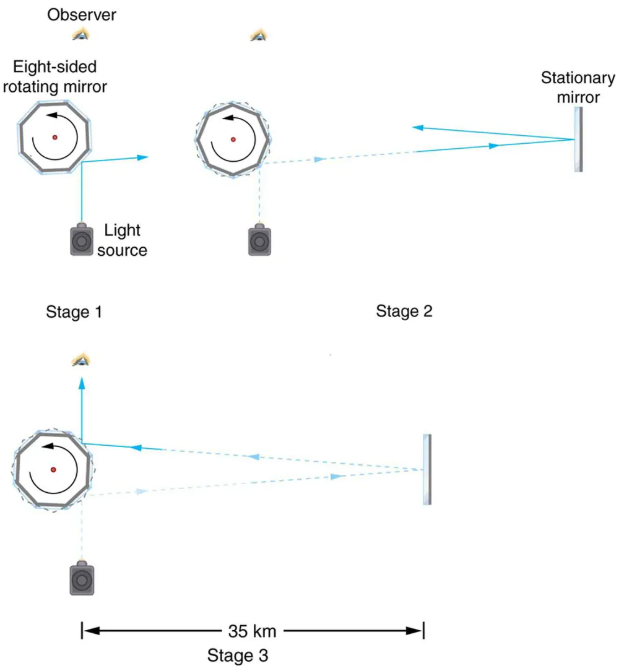
\includegraphics[width=4.5cm]{fig/c_meas.png}
\end{center}
\end{column}
\end{columns}
\end{frame}

\begin{frame}\frametitle{Refraction}
The changing of a light ray’s direction (loosely called bending) when it passes through variations in matter is called refraction.

\begin{center}
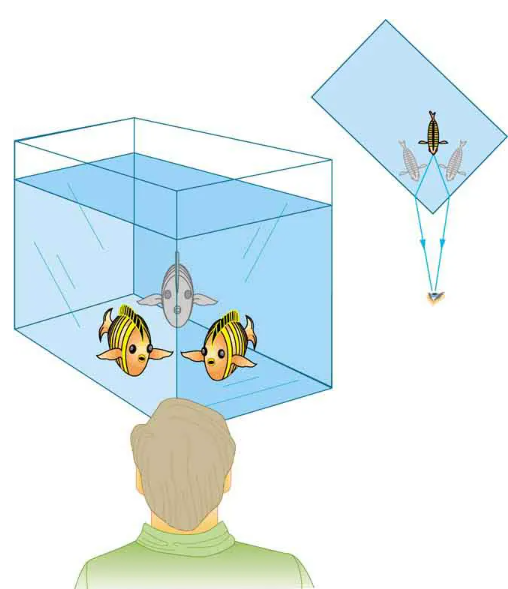
\includegraphics[width=5cm]{fig/fish.png}
\end{center}

\end{frame}


\begin{frame}\frametitle{Index of Refraction}

\begin{columns}
\begin{column}{6.5cm}
The speed of flight depends strongly on the type of material. We define the index of refraction ($n$) as

\begin{center}
$n = \frac{c}{v}$
\end{center}

where $v$ is the speed of light in the material and $c$ is the speed of light in a vacuum.
\end{column}
\begin{column}{5cm}
\begin{center}
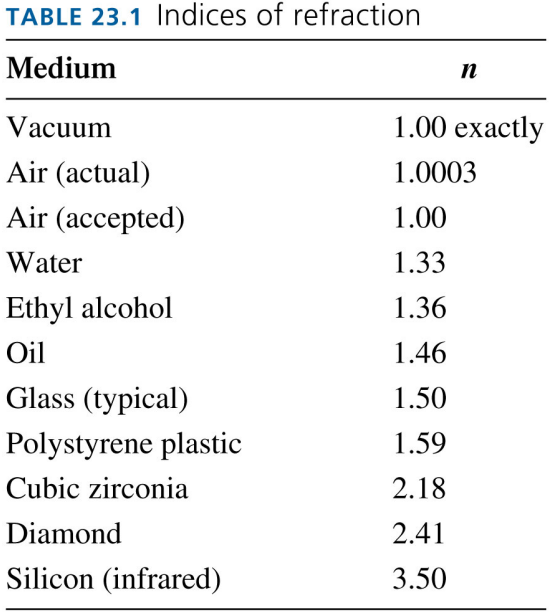
\includegraphics[width=5cm]{fig/n_table.png}
\end{center}
\end{column}
\end{columns}
\end{frame}

\begin{frame}\frametitle{Snell's Law}


\begin{center}
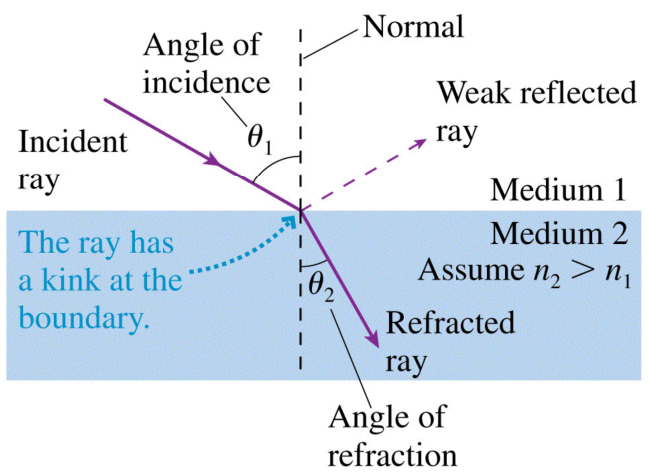
\includegraphics[width=6cm]{fig/snell.png}
\end{center}

\begin{center}
Snell's Law: $n_1 \sin{\Theta_1} = n_2 \sin{\Theta_2}$
\end{center}


\end{frame}

\section{Polarization}

\begin{frame}\frametitle{Electromagnetic Wave}

\begin{center}
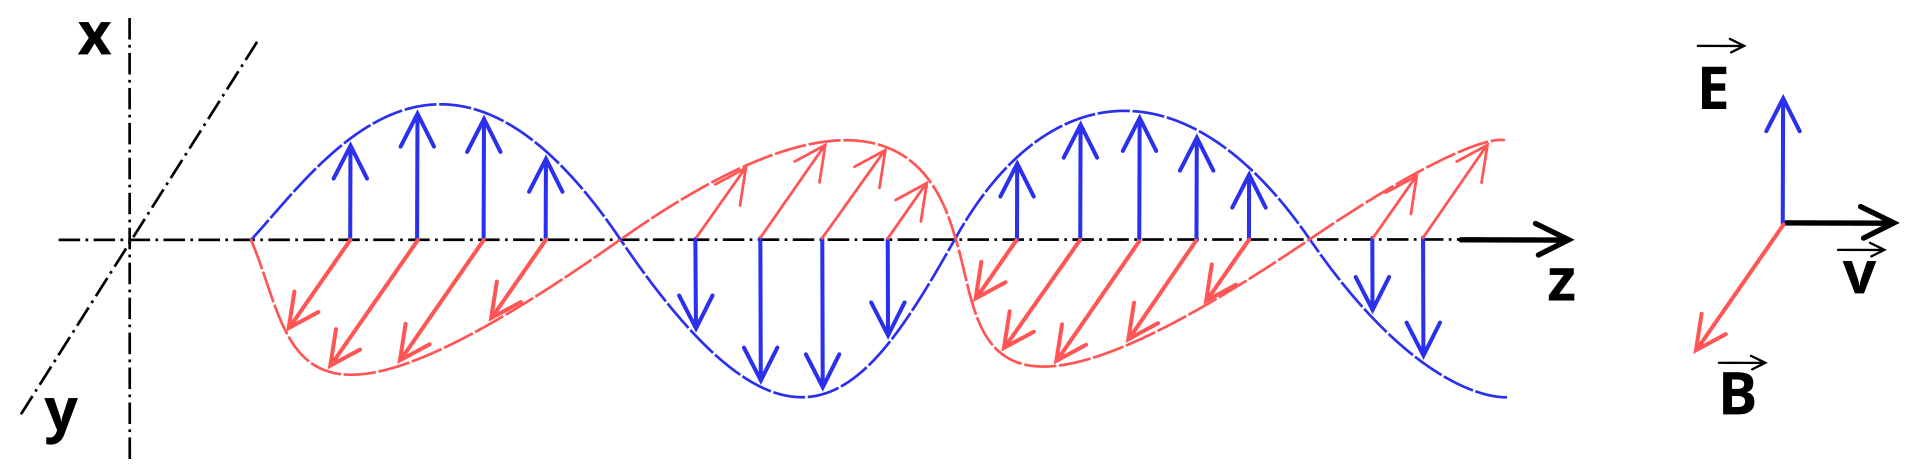
\includegraphics[width=6cm]{fig/em_wave.png}
\end{center}

An Electromagnetic (EM) wave is a transverse wave where the electric and magnetic fields are perpendicular to each other and to the direction of propagation. 

\begin{itemize}
\item Light is called unpolarized if the direction of this electric field fluctuates randomly in time. 
\item If the direction of the electric field of light is well defined, it is called polarized light. 
\end{itemize}

\end{frame}



\begin{frame}\frametitle{Linear Polarization}

We define the direction of polarization to be the direction parallel to the electric field.

\begin{center}
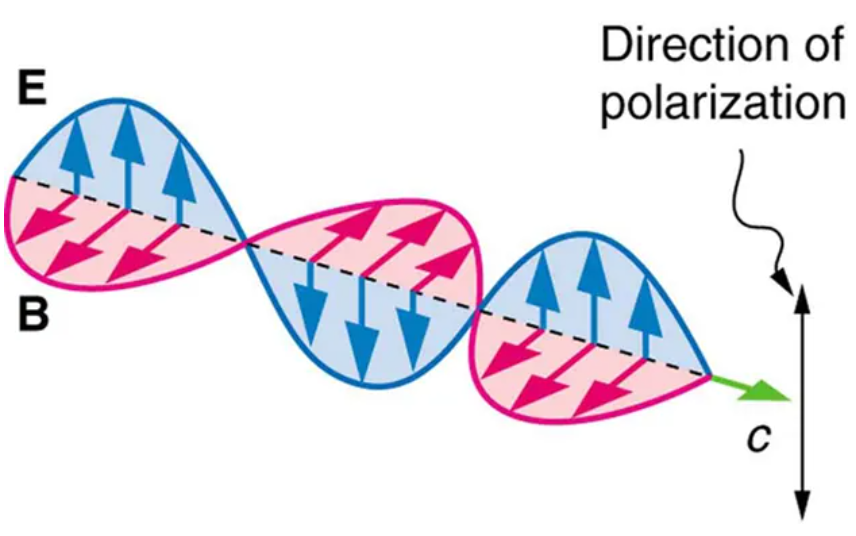
\includegraphics[width=6cm]{fig/polarization1.png}
\end{center}

\end{frame}

\section{Light - a particle or a wave}

\begin{frame}\frametitle{Corpuscular Theory of Light}

In 1675, Sir Isaac Newton hypothesized that light was made up corpuscules (small particles) with the size/mass of the corresponding to different colors. 

\begin{columns}
\begin{column}{3.5cm}
\begin{center}
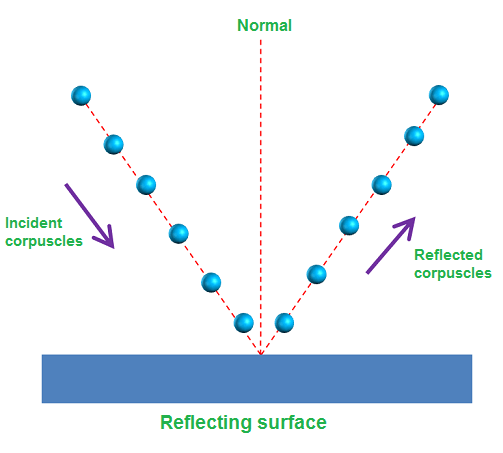
\includegraphics[width=3cm]{fig/corpReflect.png}
\end{center}
\end{column}

\begin{column}{3.5cm}
\begin{center}
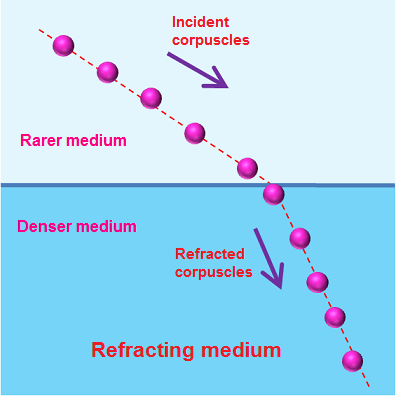
\includegraphics[width=3cm]{fig/corpRefract.png}
\end{center}
\end{column}

\begin{column}{3.5cm}
\begin{center}
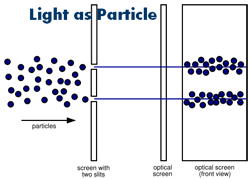
\includegraphics[width=3cm]{fig/corpDoubleSlit.png}
\end{center}
\end{column}
\end{columns}
\end{frame}

\begin{frame}\frametitle{Huygens Principle}
\begin{columns}
\begin{column}{3cm}
\begin{center}
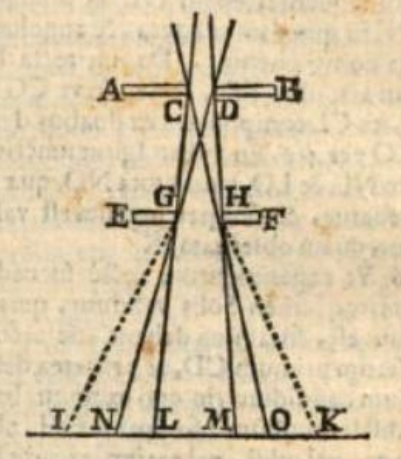
\includegraphics[width=2cm]{fig/grimaldi.png}

\vspace{0.5cm}

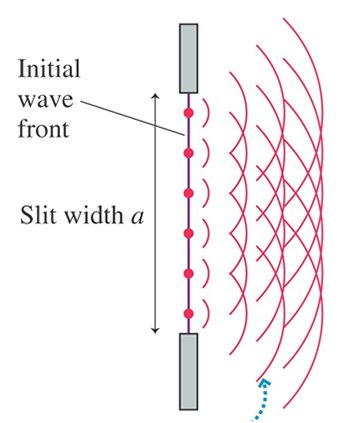
\includegraphics[width=2cm]{fig/huygens.png}

\end{center}
\end{column}

\begin{column}{8cm}
\begin{itemize}
\item Francesco Maria Grimaldi (mid-1600's) made accurate observations of the diffraction of light.

\vspace{0.5cm}

\item In 1678, Christian Huygens, in order to explain the diffraction of light, proposed that every point on a wavefront (of light) is a wavelet that spreads.
\end{itemize}
\end{column}
\end{columns}

\end{frame}


\begin{frame}\frametitle{Fresnel and Young}
\begin{columns}
\begin{column}{3cm}
\begin{center}
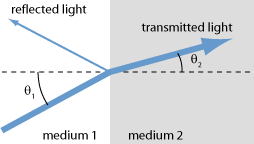
\includegraphics[width=3cm]{fig/fresnel.png}

\vspace{0.5cm}

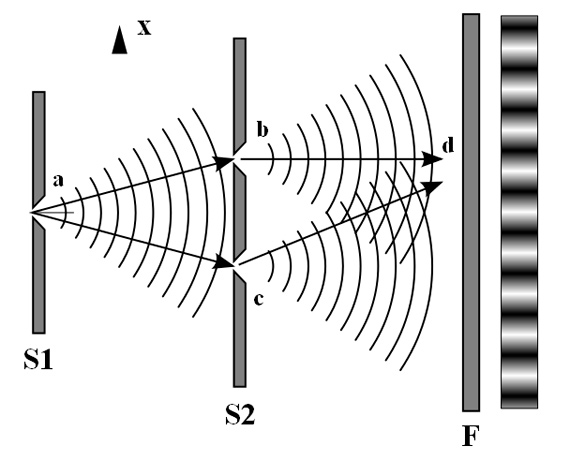
\includegraphics[width=3cm]{fig/youngDoubleSlit.jpg}

\end{center}
\end{column}

\begin{column}{8cm}
\begin{itemize}
\item In 1815, Augistine Jean Fresnel devleoped the laws of reflection and refraction.

\vspace{0.5cm}

\item And, in 1817, Thomas Young calculated the wavelength of light
\end{itemize}
\end{column}
\end{columns}

\end{frame}

\begin{frame}\frametitle{Maxwell's Equations: Electric $\vec{E}$ and Magnetic $\vec{B}$ Fields}
In 1864, James Clerk Maxwell predicted electromagnetic waves
\begin{itemize}
\item Gauss's Law: $\nabla \cdot \vec{E} = \frac{\rho}{\epsilon_0}$, where ${\rho}$ is enclosed charge
\item Guass's Law for Magnets: $\nabla \cdot \vec{B} = 0$
\item Farday's Law: $\nabla \times \vec{E} = -\frac{\partial \vec{B}}{\partial t}$
\item Ampere's Law: $\nabla \times \vec{B} = \mu_0 \vec{J} + \mu_0 \epsilon_0 \frac{\partial \vec{E}}{\partial t}$
\end{itemize}

where \newline
$\mu_0 = 4 \pi*10^{-7} \frac{F}{m}$ and 
$\epsilon_0 = 8.85*10^{-12} \frac{N m^2}{C}$ \newline

Maxwell noted that the speed of the electromagnetic wave is equal to the speed of light:


$\frac{1}{\sqrt{\mu_0 \epsilon_0}}= \frac{1}{\sqrt{4 \pi*10^{-7} \cdot 8.85*10^{-12}}} = 2.99*10^{8} \frac{m}{s} = c$
\end{frame}

\section{Intro to Quantum Phenomenon}

\begin{frame}\frametitle{Let there be light}

\end{frame}

\section{What is a Qubit}

\begin{frame} \frametitle{Bit vs Qubit}
\begin{center}
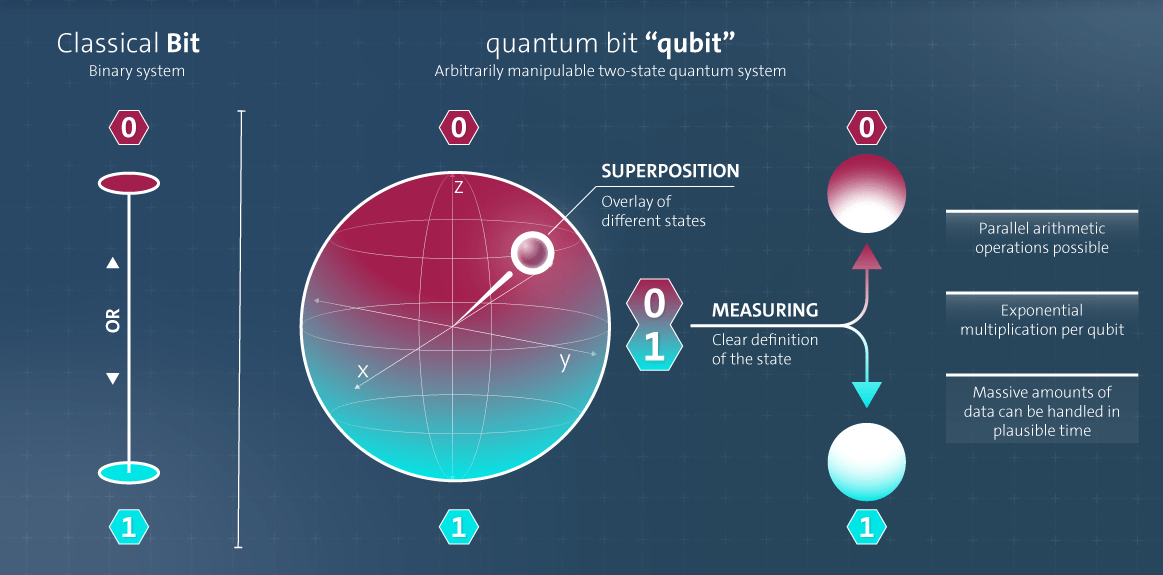
\includegraphics[width=11cm]{fig/bitQubit.png}
\end{center}

\end{frame}

\section{Quantum Computing}

\begin{frame}\frametitle{Types of Quantum Computers}
\begin{itemize}
\item Superconducting
\item Photonic
\item Neutral Atom
\item Trapped Ion
\item Quantum Dots
\item Diamond Nitrogen Vacancies
\end{itemize}
\end{frame}

\begin{frame}\frametitle{Quantum Computing: Superconducting}
One of the most popular types of quantum computers is a superconducting qubit quantum computer. Usually made from superconducting materials, these quantum computers utilize tiny electrical circuits to produce and manipulate qubits. When using superconducting qubits, gate operations can be performed quickly.

Companies actively researching and manufacturing superconducting quantum computers include Google, IBM, IQM and Rigetti Computing to name just a few.
\end{frame}


\begin{frame}\frametitle{Quantum Computing: Photonics}
These types of quantum computers use photons (particles of light) to carry and process quantum information. For large-scale quantum computers, photonic qubits are a promising alternative to trapped ions and neutral atoms that require cryogenic or laser cooling.
\end{frame}


\begin{frame}\frametitle{Quantum Computing: Neutral Atom}
Quantum computing based on neutral atoms involves atoms suspended in an ultrahigh vacuum by arrays of tightly focused laser beams called optical tweezers, though not all neutral atom companies use optical tweezers. Neutral atom quantum computers are less sensitive to stray electric fields, which makes them a good option for quantum processors.
\end{frame}


\begin{frame} \frametitle{Trapped Ions}
\begin{center}
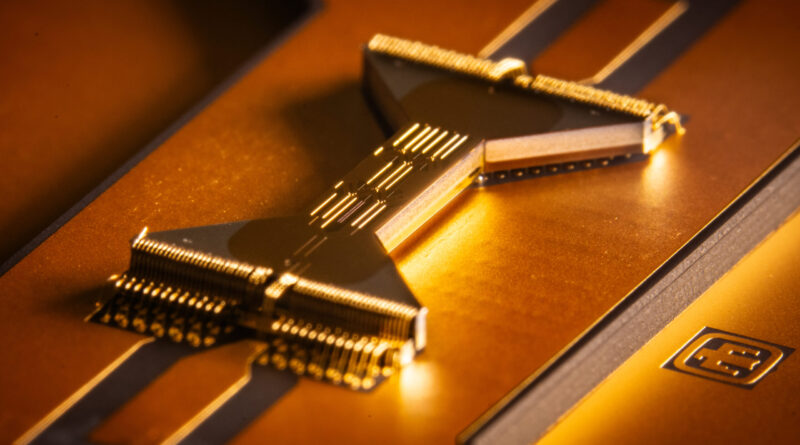
\includegraphics[width=5cm]{fig/qscoutTrappedIon.jpg}
\end{center}

A trapped ion quantum computer involves using atoms or molecules with a net electrical charge known as “ions” that are trapped and manipulated using electric and magnetic fields to store and process quantum information. As trapped ions can be isolated from their environment, they are useful for precision measurements and other applications requiring high levels of stability and control. Also, the qubits can remain in a superposition state for a long time before becoming decoherent.

Representing the trapped ions community of companies in the quantum space, we have Quantinuum (a company that came out of the merger between Cambridge Quantum Computing and Honeywell Quantum Solutions), IonQ, Quantum Factory, Alpine Quantum Technologies, eleQtron amongst others

\end{frame}


\begin{frame}\frametitle{Quantum Computing: Quantum Dots}
A quantum dot quantum computer uses silicon qubits made up of pairs of quantum dots. In theory for quantum computers, such ‘coupled’ quantum dots could be used as robust quantum bits, or qubits.

Companies focused on this area include Diraq, Siquance and Quantum Motion.
\end{frame}

\begin{frame}\frametitle{Quantum Computing: NV Diamond}

\end{frame}



\end{document}
